% --------------------------------------------------------------------------------

\begin{exercise}

Sei $\Omega \subset \R^n$ ein beschränktes Gebiet und $u$ eine klassische Lösung des parabolischen Problems

\begin{align*}
  \begin{cases}
      u_t - \Delta u + \gamma u = 0 & \text{in } \Omega \times (0,\infty), \\
      u = 0 & \text{auf } \partial\Omega \times (0,\infty), \\
      u = u_0 & \text{auf } \Omega \times \{t = 0\},
  \end{cases}
\end{align*}

wobei $u_0 \in C_0(\Omega)$ und $\gamma > 0$.
Zeigen Sie, dass

\begin{enumerate}[label = (\roman*)]
  \item $\norm[L^2(\Omega)]{u(\cdot, t)} \leq C_2 \exp(-(\lambda_1 + \gamma)t)$ für $t > 0$,
  \item $\abs{u(x, t)} \leq C_\infty \exp(-\gamma t)$ für $(x, t) \in \Omega \times (0, \infty)$,
\end{enumerate}

wobei $\lambda_1 > 0$ der kleinste Eigenwert des \textit{Laplace}-Operators $-\Delta$ und $C_2, C_\infty$ positive Konstanten sind.

\end{exercise}

% --------------------------------------------------------------------------------

\begin{solution}

\phantom{}

\begin{tcolorbox}[standard jigsaw, opacityback = 0]
  \center
  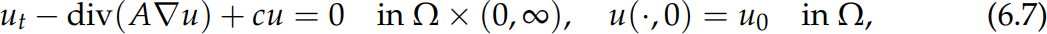
\includegraphics[width = 0.75 \textwidth]{PDEs/PDEs_-_(6-7).png} \\
  \vspace{0.1 cm}
  \hspace{3 cm}
  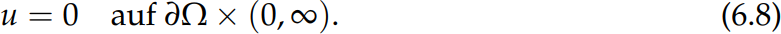
\includegraphics[width = 0.55 \textwidth]{PDEs/PDEs_-_(6-8).png}
\end{tcolorbox}

\begin{center}
  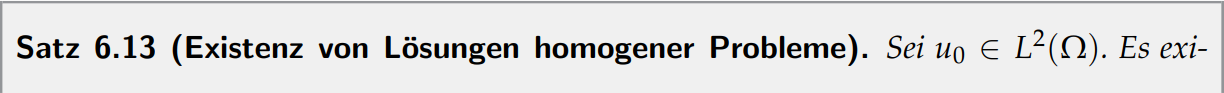
\includegraphics[width = 0.75 \textwidth]{PDEs/PDEs_-_Satz_6-13-1_(Existenz_von_Loesungen_homogener_Probleme).png} \\
  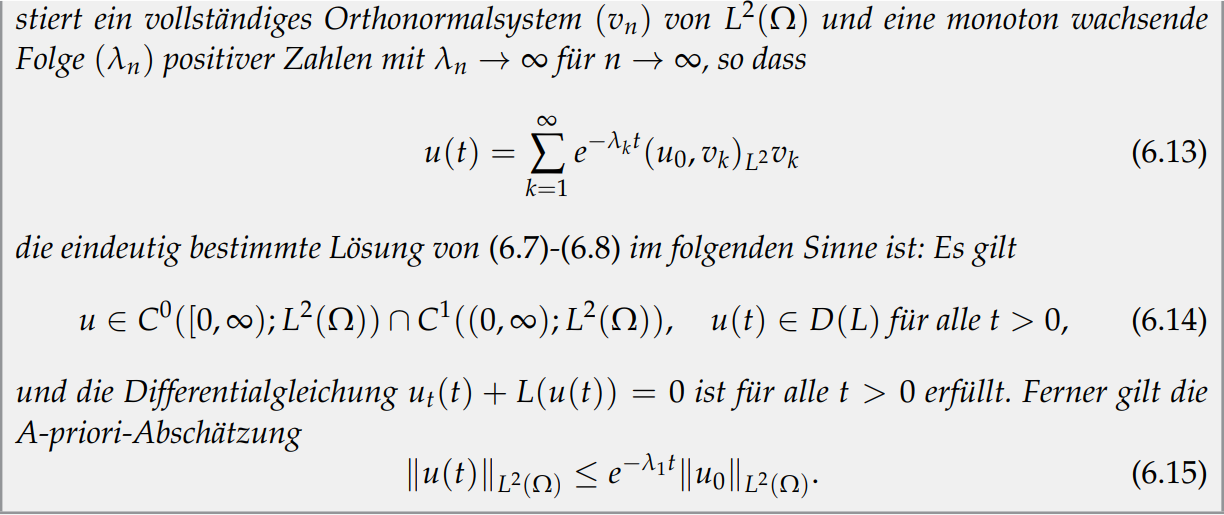
\includegraphics[width = 0.75 \textwidth]{PDEs/PDEs_-_Satz_6-13-2_(Existenz_von_Loesungen_homogener_Probleme).png}
\end{center}

\begin{enumerate}[label = (\roman*)]

  \item Wir behaupten, dass $\lambda_1 + \gamma$ der kleinste Eigenwert von $L := -\Delta + \gamma$ ist.
  Angenommen, $\tilde \lambda_1 < \lambda_1 + \gamma$ wäre ein kleinerer Eigenwert.
  Sei $\tilde v_1$ der zugehörige Eigenvektor.

  \begin{align*}
    & \implies
    \tilde \lambda_1 \tilde v_1
    =
    L \tilde v_1
    =
    (-\Delta + \gamma) \tilde v_1
    =
    -\Delta \tilde v_1 + \gamma \tilde v_1 \\
    & \implies
    (\tilde \lambda_1 - \gamma) \tilde v_1
    =
    -\Delta \tilde v_1
  \end{align*}

  Damit wäre aber $\tilde \lambda_1 - \gamma$ ein kleinerer Eigenwert von $-\Delta$ als $\lambda_1$.
  Widerspruch!

  \begin{align*}
    \tilde \lambda_1
    <
    \lambda_1 + \gamma
    \implies
    \tilde \lambda_1 - \gamma
    <
    \lambda_1
  \end{align*}

  Weil nun $\lambda_1 + \gamma$ tatsächlich der kleinste Eigenwert von $L$ ist, folgt die Behauptung aus Satz 6.13 (Existenz von Lösungen homogener Probleme).

  \begin{align*}
    \implies
    \norm[L^2]{u(\cdot, t)}
    =
    \norm[L^2(\Omega)]{u(t)}
    \stackrel
    {
      \mathrm{6.13}
    }{\leq}
    e^{-(\lambda_1 + \gamma) t}
    \underbrace
    {
      \norm[L^2(\Omega)]{u_0}
    }_{
      =: C_2
    }
  \end{align*}

  \item Die Eigenwerte von $L$ sind genau die Eigenwerte von $-\Delta$, um $\gamma$ verschoben.

  \begin{itemize}

    \item
    [\enquote{$\implies$}:]

    Sei $(\lambda, v)$ Eigenpaar von $-\Delta$, dann ist $(\lambda + \gamma, v)$ Eigenpaar von $L$.

    \begin{align*}
      (\lambda + \gamma) v
      =
      \lambda v + \gamma v
      =
      -\Delta v + \gamma v
      =
      (-\Delta + \gamma) v
      =
      L v
    \end{align*}

    \item
    [\enquote{$\impliedby$}:]

    Sei $\tilde \lambda, \tilde v$ Eigenpaar von $L$, dann ist $(\tilde \lambda - \gamma, \tilde v)$ Eigenpaar von $-\Delta$.

    \begin{align*}
      (\tilde \lambda - \gamma) \tilde v
      =
      \tilde \lambda - \gamma \tilde v
      =
      L \tilde v - \gamma \tilde v
      =
      (-\Delta + \gamma) \tilde v - \gamma \tilde v
      =
      -\Delta \tilde v + \gamma \tilde v - \gamma \tilde v
      =
      -\Delta \tilde v
    \end{align*}

  \end{itemize}

  Sei $\tilde u$ Lösung der PDE mit $\gamma = 0$.
  Wir betrachten die Darstellung (6.13) aus Satz 6.13 (Existenz von Lösungen homogener Probleme) für $\tilde u$.

  \begin{align*}
    \implies
    \Forall x \in \Omega:
    \tilde u(x, t)
    \begin{cases}
      \xrightarrow{t \to 0}      u_0, \\
      \xrightarrow{t \to \infty} 0,
    \end{cases}
    \quad
    \Forall x \in \partial \Omega:
    \tilde u(x, t)
    =
    \begin{cases}
      u_0(0) = 0, & t = 0, \\
      0,          & t \in (0, \infty)
    \end{cases}
  \end{align*}

  Weil $\tilde u \in C^2$ stetig ist, also auch beschränkt.

  \begin{multline*}
    \implies
    \abs{u(x, t)}
    \stackrel
    {
      \mathrm{(6.13)}
    }{=}
    \abs
    {
      \sum_{k=1}^\infty
      e^{-(\lambda_k + \gamma) t}
      (u_0, v_k)_{L^2}
      v_k(x)
    }
    =
    e^{-\gamma t}
    \abs
    {
      \sum_{k=1}^\infty
      e^{-\lambda_k t}
      (u_0, v_k)_{L^2}
      v_k(x)
    } \\
    \stackrel
    {
      \mathrm{(6.13)}
    }{=}
    e^{-\gamma t}
    \abs{\tilde u(x, t)}
    \leq
    e^{-\gamma t}
    \underbrace
    {
      \sup_{(y, s) \in \Omega \times (0, \infty)}
      \abs{\tilde u(y, s)}
    }_{
      =: C_\infty
    }
  \end{multline*}

\end{enumerate}

\end{solution}

% --------------------------------------------------------------------------------
